
\msection{CROW: Code Randomization of WebAssembly}
\label{section:crow}
\renewcommand{\tool}{CROW\xspace}

This section details CROW \cite{CROW}, represented as the red squared tooling in \autoref{fig:approach_landscape}. 
CROW is designed to produce functionally equivalent \wasm variants from the output of an LLVM front-end, utilizing a custom Wasm LLVM backend.

\autoref{diagrams:crow} illustrates CROW's workflow in generating program variants, a process compound of two core stages: \textit{exploration} and \textit{combination}. 
During the \textit{exploration} stage, CROW processes every instruction within each function of the LLVM input, creating a set of functionally equivalent code variants. 
This process ensures a rich pool of options for the subsequent stage.
In the \textit{combination} stage, these alternatives are assembled to form diverse LLVM IR variants, a task achieved through the exhaustive traversal of the power set of all potential combinations of code replacements. 
The final step involves the custom Wasm LLVM backend, which compiles the crafted LLVM IR variants into \wasm binaries. 


\begin{figure*}[h]
    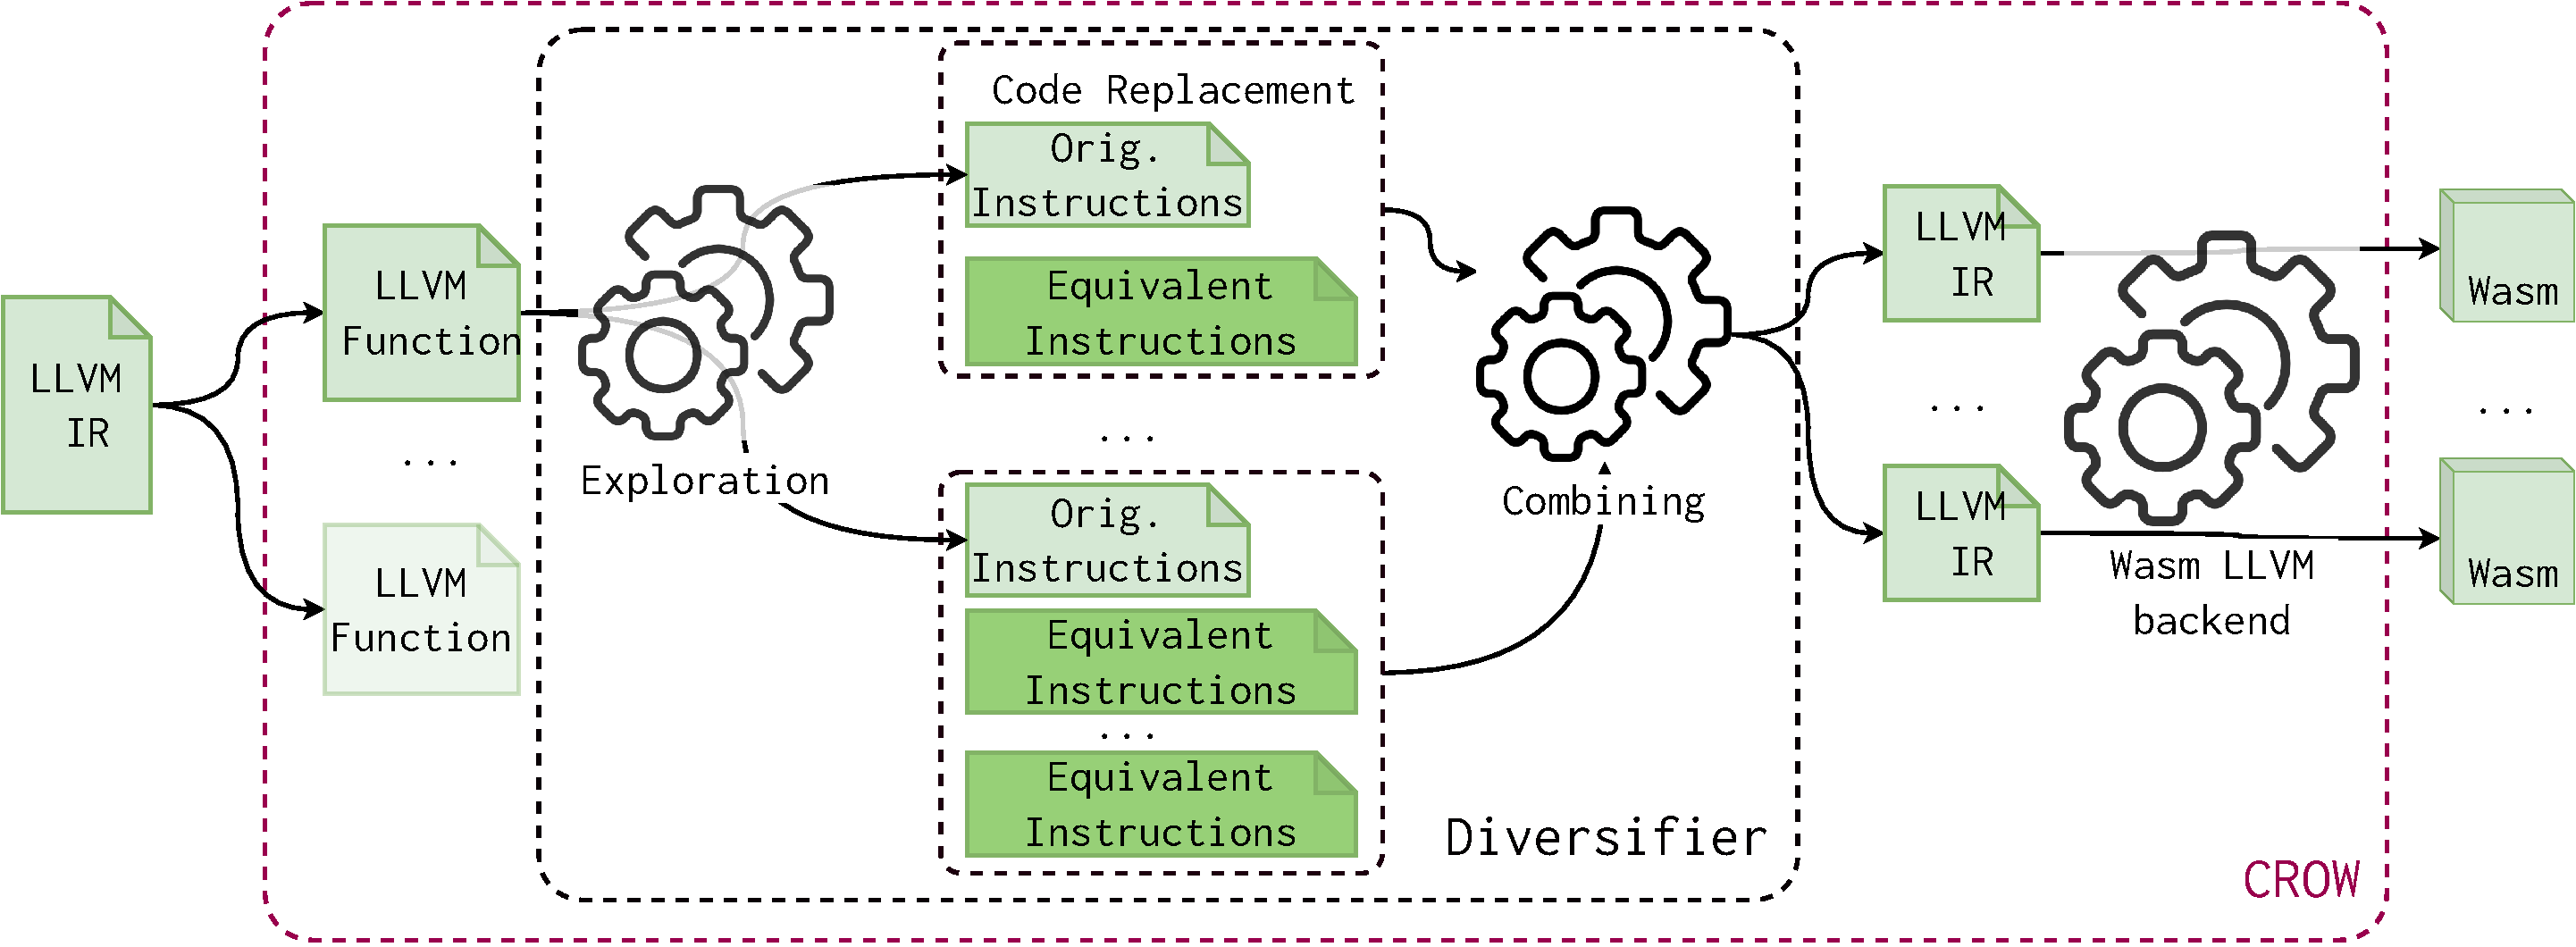
\includegraphics[width=\linewidth]{diagrams/generation/crow.drawio.pdf}
    \caption{CROW components following the diagram in \autoref{fig:approach_landscape}. CROW takes LLVM IR to generate functionally equivalent code replacements. Then, CROW assembles program variants by combining them. Figure taken from \cite{Lic}.}
    \label{diagrams:crow}
\end{figure*}


%\emph{Exploration}
\msubsection{Enumerative synthesis}

The cornerstone of CROW's exploration mechanism is its code replacement generation strategy, which is inspired by the superdiversifier methodology proposed by Jacob \etal~\cite{jacob2008superdiversifier}. 
The search space for generating variants is delineated through an enumerative synthesis process (see \mnameref{enumerative_synthesis}{artificial_diversity}), which systematically produces all possible code replacements for each data flow graph that can be constructed from the original program. 
If a code replacement is identified to function identically to the original program, it is reported as a functionally equivalent variant.
This equivalence is confirmed using a theorem solver for rigorous verification.

CROW is developed by extending the enumerative synthesis implementation found in Souper \cite{Sasnauskas2017Souper:Superoptimizer}, an LLVM-based superoptimizer. 
Specifically, CROW constructs a Data Flow Graph(DFG) for each LLVM instruction that returns an integer. 
Subsequently, it generates all viable expressions derived from a selected subset of the LLVM Intermediate Representation.
The enumerative synthesis process incrementally generates code replacements, starting with the simplest expressions (those composed of a single instruction) and gradually increasing in complexity. 
The exploration process continues either until a timeout occurs or the size of the generated replacements exceeds a predefined threshold.


% Boosting the geneation of variants
CROW is carefully designed to boost the generation of variants as much as possible.
First, we disable the majority of the pruning strategies.
Instead of preventing the generation of commutative operations during the search, CROW still uses such transformation as a strategy to generate program variants. 
Second, CROW applies code transformations independently. 
For instance, if a suitable replacement is identified that can be applied at $N$ different locations in the original program, CROW will generate $2^N$ distinct program variants, i.e., the power set of applying the transformation or not to each location. 
This approach leads to a combinatorial explosion in the number of available program variants, especially as the number of possible replacements increases.
Third, we remove all built-in optimizations in the LLVM backend that could reverse Wasm variants, i.e., we disable all optimizations in the \wasm\ backend that could reverse the CROW transformations

Notice that, the search space increases exponentially with the number of language instructions used for enumerative synthesis. 
To mitigate this issue, we prevent CROW from synthesizing instructions without correspondence in the \wasm\ backend.
For example, removing LLVM instructions without corresponding \Wasm instructions effectively reduces the search space.

% The full spectrumg
Leveraging the ascending nature of its enumerative synthesis process, CROW is capable of creating variants that may outperform the original program in both size and efficiency. 
For instance, the first functionally equivalent transformation identified is typically the most optimal in terms of code size. 
This approach offers developers a range of performance options, allowing them to balance between diversification and performance without compromising the latter.

%\vspace{-1cm}

\msubsection{Constant inferring}
\label{CROW:constant_inferring}
CROW inherently introduces a transformation strategy called \emph{constant inferring}, which significantly expands the variety of \Wasm program variants. 
Specifically, CROW identifies segments of code that can be simplified into a single constant assignment, with a particular focus on variables that control branching logic. 
After applying this \emph{constant inferring} technique, the resulting program diverges substantially from the original program structure. 
This is crucial for diversification efforts, as one of the primary objectives is to create variants that are as distinct as possible from the original code (see \autoref{measuring_diversification}). 
In essence, the more divergent the variant, the more challenging it becomes to trace it back to its original form.
% This transformation is especially useful for generating \wasm variants that are highly preserved after the JIT compilation of further compilers.




Let us illustrate the case with an example.
The Babbage problem code in \autoref{babbage} is composed of a loop that stops when it discovers the smallest number that fits with the Babbage condition in Line 4.


{


\begin{minipage}[t]{0.43\linewidth}
        \lstset{
        language=C,
        style=CStyle,
        columns=fullflexible,
        breaklines=true,
        belowcaptionskip=30pt,
        abovecaptionskip=1pt,
        columns=fullflexible,
        breaklines=true, 
        caption={Babbage problem. Taken from \cite{Lic}.},
        frame=b,
        captionpos=b,
        numbers=none,
        label=babbage,
        postbreak=\mbox{\textcolor{red}{$\hookrightarrow$}\space}
    } 
    \begin{lstlisting}[numbers=left]
    int babbage() {
        int current = 0,
            square;
        while ((square=current*current) % 1000000 != 269696) {
            current++;
        }
        printf ("The number is %d\n", current);
        return 0 ;
    }
    \end{lstlisting}
\end{minipage}\hfill
\begin{minipage}[t]{0.44\linewidth}
        \lstset{
        language=C,
        style=CStyle,
        columns=fullflexible,
        breaklines=true,
        belowcaptionskip=3pt,
        abovecaptionskip=1pt,
        columns=fullflexible,
        breaklines=true, 
        frame=b,
        numbers=none,
        captionpos=b,
        caption={Constant inferring transformation over the original Babbage problem in \autoref{babbage}. Taken from \cite{Lic}.},
        label=inferring,
        postbreak=\mbox{\textcolor{red}{$\hookrightarrow$}\space}
    } 
    \begin{lstlisting}[]
int babbage() {
    @int current = 25264;@
    
    




    printf ("The number is %d\n", current);
    return 0 ;
}
    \end{lstlisting}
\end{minipage}
}

% llvm-opt: rool unroll
CROW deals with this case, generating the program in \autoref{inferring}. It infers the value of \texttt{current} in Line 2 such that the Babbage condition is reached\footnote{
    In theory, this value can also be inferred by unrolling the loop the correct number of times with the LLVM toolchain.
    However, standard LLVM tools cannot unroll the \texttt{\textbf{while}}-loop because the loop count is too large.}. 
Therefore, the condition in the loop will always be false. Then, the loop is dead code and is removed in the final compilation. 
The new program in \autoref{inferring} is remarkably smaller and faster than the original code. Therefore, it offers differences both statically and at runtime\footnote{ Notice that for the sake of illustration, we show both codes in the C language; this process inside CROW is performed directly in LLVM IR.}.
%  Also, notice that the two programs in the example follow the definition of \emph{functional equivalence} discussed in \autoref{sota:sota}.}



\msubsection{Exemplifying CROW}
\label{section:crow:example}
%In \autoref{section:crow} we describe the main components and contributions of CROW. In this section we instantiate the workflow presented in \autoref{workflow} from the input of an example C code to the generation of a pool of \wasm\ program variants.

Let us illustrate how CROW works with the example code in \autoref{CExample}. The \texttt{f} function calculates the value of $2 * x + x$ where \texttt{x} is the input for the function.  CROW compiles this source code and generates the intermediate LLVM bitcode in the leftmost part of \autoref{example:crow:original:llvm}. CROW potentially finds two integers returning instructions to look for variants, as the rightmost part of \autoref{example:crow:original:llvm} shows.

% snippet of code showing the detection of code blocks
\begin{minipage}[t]{.9\linewidth}
%\begin{code}
    \lstset{
        language=C,
        basicstyle=\small\ttfamily,captionpos=b,caption={C function that calculates the quantity $2x + x$.},label=CExample, frame=b}
    
    \begin{lstlisting}[style=CStyle]
int f(int x) { 
    return 2 * x + x; 
}    
    \end{lstlisting}
%\end{code}
\end{minipage}

\lstdefinelanguage{LLVM}
    {morekeywords={i32,mul,align,nsw,add,load,store,define,br, ret, shl, ret},
    sensitive=false,
    morecomment=[l]{;},
    morecomment=[s]{;}{;},
    morestring=[b],
}

\lstdefinestyle{nccode}{
    numbers=left,
    tabsize=4,
    showspaces=false,
    breaklines=true, 
    showstringspaces=false,
    moredelim=**[is][{\btHL[fill=black!10]}]{`}{`},
    moredelim=**[is][{\btHL[fill=celadon!40]}]{!}{!}
}
\lstset{
    language=LLVM,
    style=nccode,
    %basicstyle=\small\ttfamily,
    columns=fullflexible,
    breaklines=true
}

\begin{minipage}[t]{0.9\linewidth}
    
    \lstset{numbers=none}
    \noindent\begin{minipage}[t]{.34\linewidth}
    \centering
    \begin{lstlisting}[xleftmargin=1em,escapechar=?]
    define i32 @f(i32) {

      %2 = mul nsw i32 %0,2
      %3 = add nsw i32 %0,%2 

      ret i32 %3
    }
    
    define i32 @main() {
      %1 = tail call i32 @f(i32 10)
      ret i32 %1
    }
    \end{lstlisting}
    \end{minipage}%\hfill%
    \begin{minipage}[t]{.32\linewidth}
        \begin{lstlisting}[xleftmargin=1em,escapechar=?]
?Replacement candidates for code\_1?

`%2 = mul nsw i32 %0,2`

!%2 = add nsw i32 %0,%0!

!%2 = shl nsw i32 %0, 1:i32!
    \end{lstlisting}
    \end{minipage}%\hfill%
    \begin{minipage}[t]{.32\linewidth}
        \lstdefinestyle{nccode}{
        tabsize=4, 
        showspaces=false,
        breaklines=true, 
        showstringspaces=false,
        moredelim=**[is][{\btHL[fill=black!10]}]{`}{`},
        moredelim=**[is][{\btHL[fill=celadon!40]}]{!}{!}
        }
        \lstset{
            language=LLVM,
            style=nccode,
            columns=fullflexible,
            breaklines=true,
            belowcaptionskip=1pt,
            abovecaptionskip=1pt,
        } 
        \begin{lstlisting}[name={B},escapechar=?]
?Replacement candidates for code\_2?

`%3 = add nsw i32 %0,%2`

!%3 = mul nsw %0, 3:i32!
        \end{lstlisting}
    \end{minipage}
    \centering
    \hrule
    \vspace{2mm}
    \captionof{lstlisting}{LLVM's intermediate representation program, its extracted instructions and replacement candidates. Gray highlighted lines represent original code, green for code replacements. }\label{example:crow:original:llvm}
\end{minipage}

\begin{minipage}[t]{.9\linewidth}
    \lstset{numbers=none}
    \noindent\begin{minipage}[t]{.5\linewidth}
    \begin{lstlisting}[xleftmargin=1em,escapechar=?]
`%2 = mul nsw i32 %0,2`
`%3 = add nsw i32 %0,%2`

!%2 = add nsw i32 %0,%0!
`%3 = add nsw i32 %0,%2`

!%2 = shl nsw i32 %0, 1:i32!
`%3 = add nsw i32 %0,%2`

    \end{lstlisting}
    \end{minipage}%\hfill%
    \begin{minipage}[t]{.5\linewidth}
        \lstdefinestyle{nccode}{
        tabsize=4, 
        showspaces=false,
        breaklines=true, 
        showstringspaces=false,
        moredelim=**[is][{\btHL[fill=black!10]}]{`}{`},
        moredelim=**[is][{\btHL[fill=celadon!40]}]{!}{!},
        moredelim=**[is][{\btHL[fill=weborange!40]}]{'}{'}
        }
        \lstset{
            language=LLVM,
            style=nccode,
            columns=fullflexible,
            breaklines=true,
            belowcaptionskip=1pt,
            abovecaptionskip=1pt,
        } 
        \begin{lstlisting}[xleftmargin=1em,escapechar=?]
'%2 = mul nsw i32 %0,2'
!%3 = mul nsw %0, 3:i32!

'%2 = add nsw i32 %0,%0'
!%3 = mul nsw %0, 3:i32!

'%2 = shl nsw i32 %0, 1:i32'
!%3 = mul nsw %0, 3:i32!

    \end{lstlisting}
    \end{minipage}
    \centering
    \hrule
    \vspace{2mm}
    \captionof{lstlisting}{Candidate code replacements combination. Orange highlighted code illustrate replacement candidate overlapping.}\label{example:crow:original:combination}
\end{minipage}


    

CROW, detects \texttt{code\_1} and \texttt{code\_2} as the enclosing boxes in the leftmost part of \autoref{example:crow:original:llvm} shows. CROW synthesizes $2 + 1$ candidate code replacements for each code respectively as the green highlighted lines show in the rightmost parts of \autoref{example:crow:original:llvm}.
The baseline strategy of CROW is to generate variants out of all possible combinations of the candidate code replacements, \ie uses the power set of all candidate code replacements.

In the example, the power set is the cartesian product of the found candidate code replacements for each code block, including the original ones, as \autoref{example:crow:original:combination} shows. The power set size results in $6$ potential function variants. Yet, the generation stage would eventually generate $4$ variants from the original program. CROW generated 4 statically different Wasm files, as \autoref{example:crow:variants:wasm} illustrates. This gap between the potential and the actual number of variants is a consequence of the redundancy among the bitcode variants when composed into one. In other words, if the replaced code removes other code blocks, all possible combinations having it will be in the end the same program. In the example case, replacing \texttt{code\_2} by \texttt{mul nsw \%0, 3}, turns \texttt{code\_1} into dead code, thus, later replacements generate the same program variants. The rightmost part of \autoref{example:crow:original:combination} illustrates how for three different combinations, CROW produces the same variant. We call this phenomenon a \emph{code replacement overlapping}.

\lstdefinestyle{nccode}{
        numbers=none,
        firstnumber=2,
        stepnumber=1,
        numbersep=10pt,
        tabsize=4, 
        showspaces=false,
        breaklines=true, 
        showstringspaces=false,
    moredelim=**[is][\btHL]{`}{`},
    moredelim=**[is][{\btHL[fill=black!10]}]{`}{`},
    moredelim=**[is][{\btHL[fill=celadon!40]}]{!}{!}
}

\lstset{
    language=WAT,
    style=nccode,
    basicstyle=\footnotesize\ttfamily,
    columns=fullflexible,
    breaklines=true
}


\begin{minipage}[t]{0.9\linewidth}
    \lstset{numbers=none}
    \noindent\begin{minipage}[t]{.45\linewidth}
    \begin{lstlisting}[xleftmargin=1em,escapechar=?]
func $f (param i32) (result i32)
   local.get 0
    `i32.const 2`
    `i32.mul`
    `local.get 0`
    `i32.add`

        \end{lstlisting}
\begin{lstlisting}[xleftmargin=1em,escapechar=?]
func $f (param i32) (result i32)
    local.get 0
    !local.get 0!
    !i32.add!
    `local.get 0`
    `i32.add`

                \end{lstlisting}
    \end{minipage}\hfill
    \noindent\begin{minipage}[t]{.45\linewidth}
\begin{lstlisting}[xleftmargin=1em,escapechar=?]
func $f (param i32) (result i32)
    local.get 0
    !i32.const 1!
    !i32.shl!
    `local.get 0`
    `i32.add`

    \end{lstlisting}
\begin{lstlisting}[xleftmargin=1em,escapechar=?]
func $f (param i32) (result i32)
    local.get 0
    !i32.const 3!
    !i32.mul!

        \end{lstlisting}
    \end{minipage}

    \centering
    \hrule
    \vspace{2mm}
    \captionof{lstlisting}{Wasm  program variants generated from program \autoref{CExample}.}\label{example:crow:variants:wasm}
\end{minipage}




\begin{tcolorbox}[title=Contribution paper and artifact,boxrule=1pt,arc=.2em,boxsep=1.0mm]
    CROW is a compiler-based approach.
    It leverages enumerative synthesis to generate functionally equivalent code replacements and assembles them into diverse \wasm program variants. 
    CROW uses SMT solvers to guarantee functional equivalence. \\
    CROW is fully presented in Cabrera-Arteaga \etal "CROW: Code Randomization of WebAssembly"
    \emph{at proceedings of Measurements, Attacks, and Defenses for the Web (MADWeb), NDSS 2021}
    \url{https://doi.org/10.14722/madweb.2021.23004}. 
    \\\\
    CROW source code is available at \url{https://github.com/ASSERT-KTH/slumps}

\end{tcolorbox}

